% numerics.tex      pdflatex ZhCvGo15
% Diffuse globally, compute locally: a cyclist tale
% Tingnan Zhang, Daniel I. Goldman and Predrag Cvitanovi\'c

%\subsection{Numerical results}
%                         was {Diffusion in the fundamental domain}
%\label{s-numerics}
\begin{table}[htbp]
	\centering
	\begin{tabular}{|r|r|r|l|l|}
		\hline
		${n_p}$ & \# cycles & $\zeta$(0,0) & $\lambda$ & D \\ 
		\hline\hline
		1      & 0      &   -    &   -  &   - \\
		2      & 24     & -0.31697 & 1.330 & 0.375\\
		3      & 64     & -0.54152 & 1.435 & 0.339\\
		4      & 168    & -0.09764 & 1.902 & 0.284\\
		5      & 516    &  0.02334 & 2.324 & 0.215\\
		6      & 1589   & -0.00481 & 1.975 & 0.133\\
		7      & 5700   & -0.01241 & 1.885 & 0.184\\
		8      & 20729  & -0.01006 & 1.785 & 0.247\\ \hline
	\end{tabular}
	\caption[Elementary cell cycle expansion results of diffusion 
	coefficient]{\label{TCELL1}
		Elementary cycle expansion results~\refeq{eq-diff-ec} computed
		Schreiber 1992 calculation\rf{CGS92} (and this paper) in the
		elementary cell.}
\end{table}

Elementary cycles and the corresponding cycle expansion calculation
results are listed in \reftab{TCELL1}. Although the diffusion
coefficient computed using elementary cycles up to $n_p = 8$ is close 
to the numerical experiment value $0.25$, the convergence is not
promising, as have pointed out in~\refref{CGS92, Morriss1994}.

\begin{table}[htbp]
	\centering
	\begin{tabular}{|r|r|r|l|l|}
		\hline
		$\period{p}$ & \# cycles & $\zeta$(0,0) & $\lambda$ & D \\ 
		\hline\hline
		1      & 5      & -0.2169759 & 1.39193 & 0.37795 \\
		2      & 10     & -0.0248233 & 1.74541 & 0.23118 \\
		3      & 33     & -0.0221962 & 1.72235 & 0.25257 \\
		4      & 108    & -0.0002192 & 1.74450 & 0.24165 \\
		5      & 373    &  0.0023463 & 1.76079 & 0.24468 \\
		6      & 1378   &  0.0096330 & 1.75610 & 0.24068 \\ 
		\hline\hline
		\multicolumn{3}{|l|}{numerical experiment}
		& 1.760   & 0.25
		\\ \hline
	\end{tabular}
	\caption[Fundamental domain cycle expansion results of diffusion 
	coefficient]{\label{TCELL2}
		Results for $w$=0.3. Calculation in the fundamental domain . 
		Gaspard 
		1992 note: ``My
		numerical estimate for the Lyapunov exponent when $w=0.3$ is
		$\lambda = 1.760 \pm 0.002$, which supports the result of this
		table.'' The numerical diffusion coefficient is calculated 
		using 
		Green-Kubol method. 
	}
\end{table}

We list the numerical results computed using the fundamental domain
orbits (Equation~\refeq{eq-fd-msd}) in \reftab{TCELL2}. Compared with
other methods, the symmetry-reduced cycle expansion method converges
the fastest, see \reftab{TCELL2} and \reffig{fig-results}A. Diffusion
coefficient computed from $\sim2\,000$ fundamental domain cycles of
topological length up to 6 converges to two significant digits, while
the elementary cell calculation needs over $\sim 10\,000$ cycles in
order to converge.

\begin{figure}
	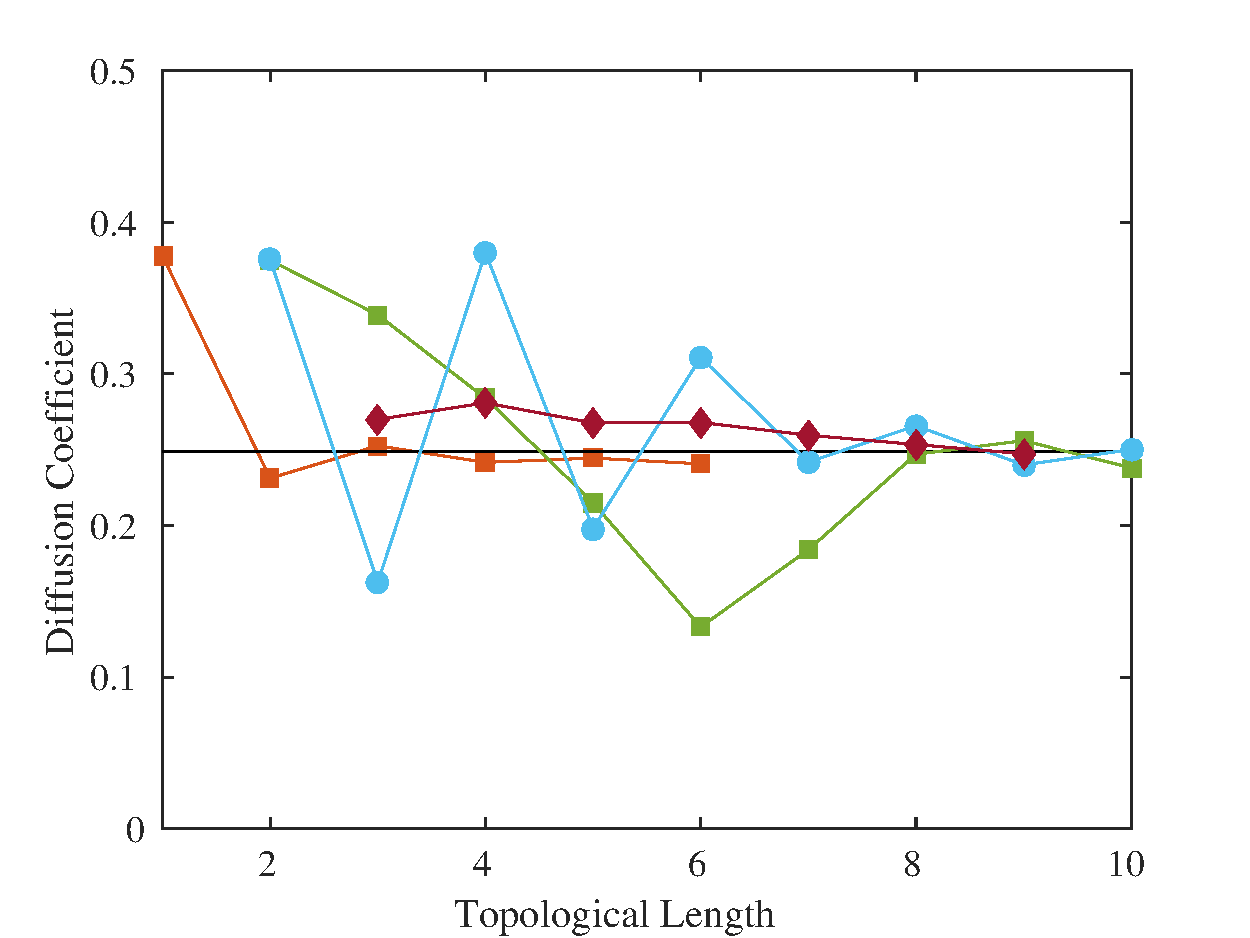
\includegraphics[width=0.5\textwidth]{diffuseCycleExpansionResults}
	\caption{\label{fig-convergence}The convergence of diffusion 
	coefficients  calculated using cycle		
		expansion in elementary cell (green squares), and fundamental 
		domain (orange squares). We also show the convergence of 
		``periodic orbit expansion'' method, with and  without Shanks 
		transformation (circles and diamonds) discussed in  
		\refref{Morriss1994}. Here $w = 0.3$.
		}
\end{figure}
\begin{figure}
	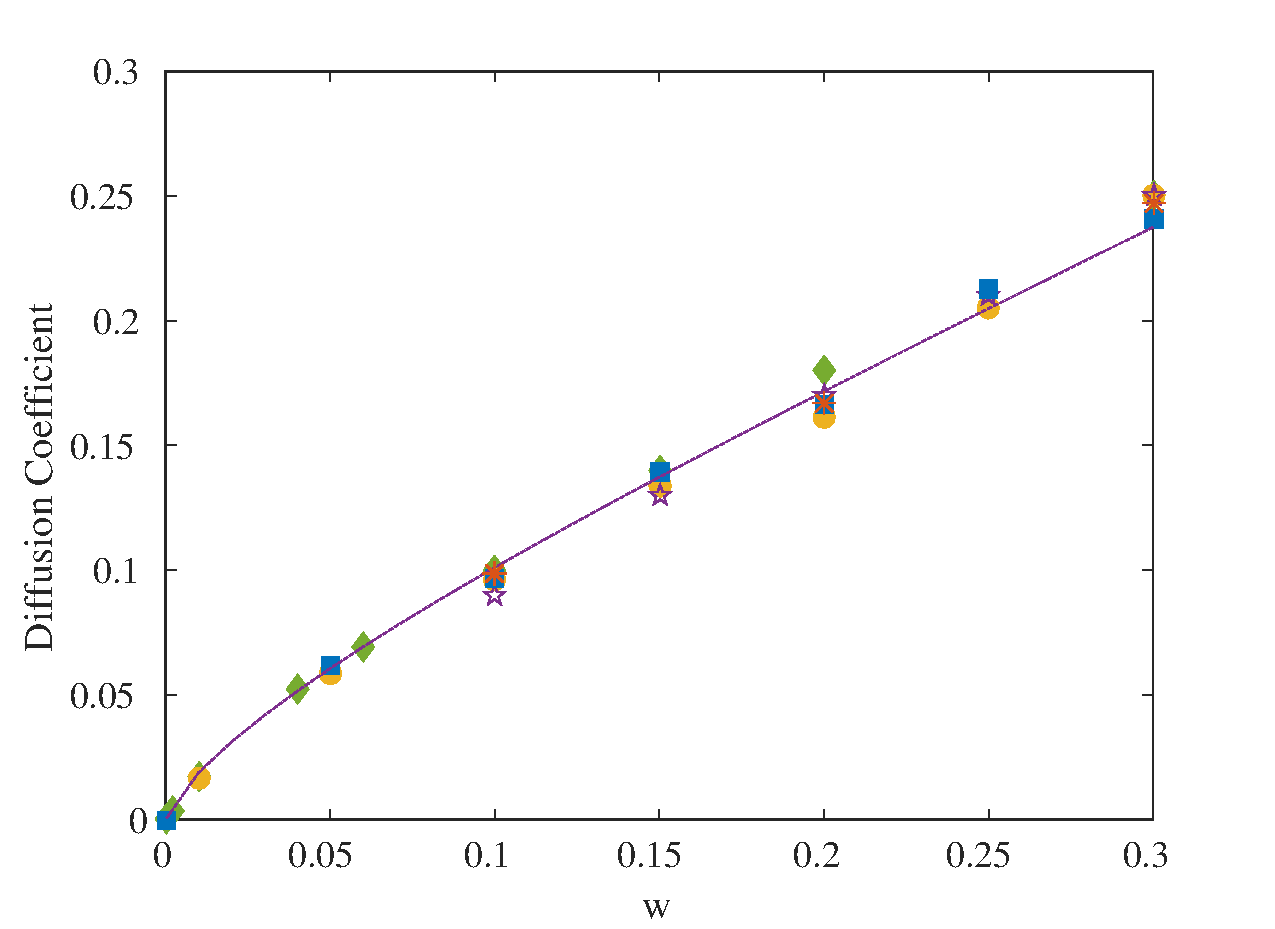
\includegraphics[width=0.5\textwidth]{diffuseDiffCoefPlot}
	\caption[Diffusion coefficients computed using cycle expansion 
	formulas]{\label{fig-results} 
		(A) The convergence of diffusion coefficients  calculated 
		using cycle
		expansion in elementary cell (green squares),  fundamental
		domain(orange squares). We  also show the convergence of 
		``periodic
		orbit expansion'' method, with and  without Shanks 
		transformation
		(circles and diamonds) discussed in  \refref{Morriss1994}. 
		Here $w =
		0.3$. (B) Diffusion coefficients as a function $w$.  Figure
		generated using data from various resources. Diamonds are 
		results
		from  Green-Kubo numerical experiments\rf{MacZwa83};
		stars\rf{BaEvCo93} and  circles\rf{GasBar95} are calculated 
		from
		escape rate; and triangles are  given by Hausdorff fractal 
		dimension
		calculation\rf{GasBar95}; dashed line  is a statistical
		approximation from\rf{AngMor12}.}
\end{figure}

We also compute the diffusion coefficient for $w = 0.05, 0.10, 0.15,
0.20, 0.25, 0.30$. The results are compared with previous numerical
experiments and a recent statistical estimation, see
\reffig{fig-results}. In Green-Kubo velocity auto-correlation method
the  diffusion coefficient can be extrapolated to the accurate
reference value $0.250$ (at $w/r=0.30$), using ensembles of
$10^6\sim10^7$ random trajectories that fly for an extensive period
($T > 20$)\rf{MacZwa83}. The number of bounces for each trajectory are
typically greater than $20$ (as compared to 6, the topological length
of longest periodic orbit we used). On the other hand, while
statistical approach yields a smooth analytical formula\rf{AngMor12},
the diffusion property in such systems is fundamentally never a 
smooth function of parameters\rf{Cristad06}. Unfortunately, for 
the 2D system we do not have enough numerical precision to monitor 
the fractal behavior of diffusion coefficient observed in 
\refref{Cristad06}. 

We have numerically computed the diffusion coefficient using the map version of the trace formula. However, if we consider the continuous flow, i.e. by replacing the discrete sum with the integral~\refeq{eq-orbitsum}, the result could be different. We find that, by our surprise,  the continuous version of the trace formula converged to lower numerical values (\reftab{TCELL3}). For any length-1 fundamental domain periodic orbit, the cycle averaged square displacement $\left\langle\vert\hat{L}_{\tp}(r,\tx)\vert^2\right\rangle_{\tp}$ is lower if we count all the points along the flight. For example, if we start at the cell boundary on the cycle $\{{\bar{0}, \underline{5}}\}$ (the bouncing mode between the nearest disks), the net displacement in full space is $0$ after we complete the fundamental domain cycle once. To the contrary, starting from the disk edge would generate a net displacement of $w$. A careful evaluation of the continuous average then produce $\left\langle\vert\hat{L}_{\tp}(1,\tx)\vert^2\right\rangle_{\tp} = w^2/3$.

Although the difference between the integral and the discrete sum vanishes when cycles grow longer, the expansion results are dominated by the shortest orbits, which contribute exponentially many times in the formula. 

\begin{table}[htbp]
	\centering
	\begin{tabular}{|r|r|r|r||}
		\hline
		$\period{p}$ & \# cycles & D (cont) & D (discrete) \\ 
		\hline\hline
		1      & 5      & 0.21597 & 0.37795 \\
		2      & 10     & 0.23557 & 0.23118 \\
		3      & 33     & 0.20404 & 0.25257 \\
		4      & 108    & 0.23073 & 0.24165 \\
		5      & 373    & 0.21379 & 0.24468 \\
		6      & 1378   & 0.21902 & 0.24068 \\ 
		\hline
	\end{tabular}
	\caption[Fundamental domain cycle expansion results of diffusion 
	coefficient]{\label{TCELL3}
		Fundamental domain cycle expansion results of diffusion 
		coefficient, computed using continuous integral (3rd column) and discrete sum (4th column). Here $w = 0.3$.
	}
\end{table}

\begin{figure}
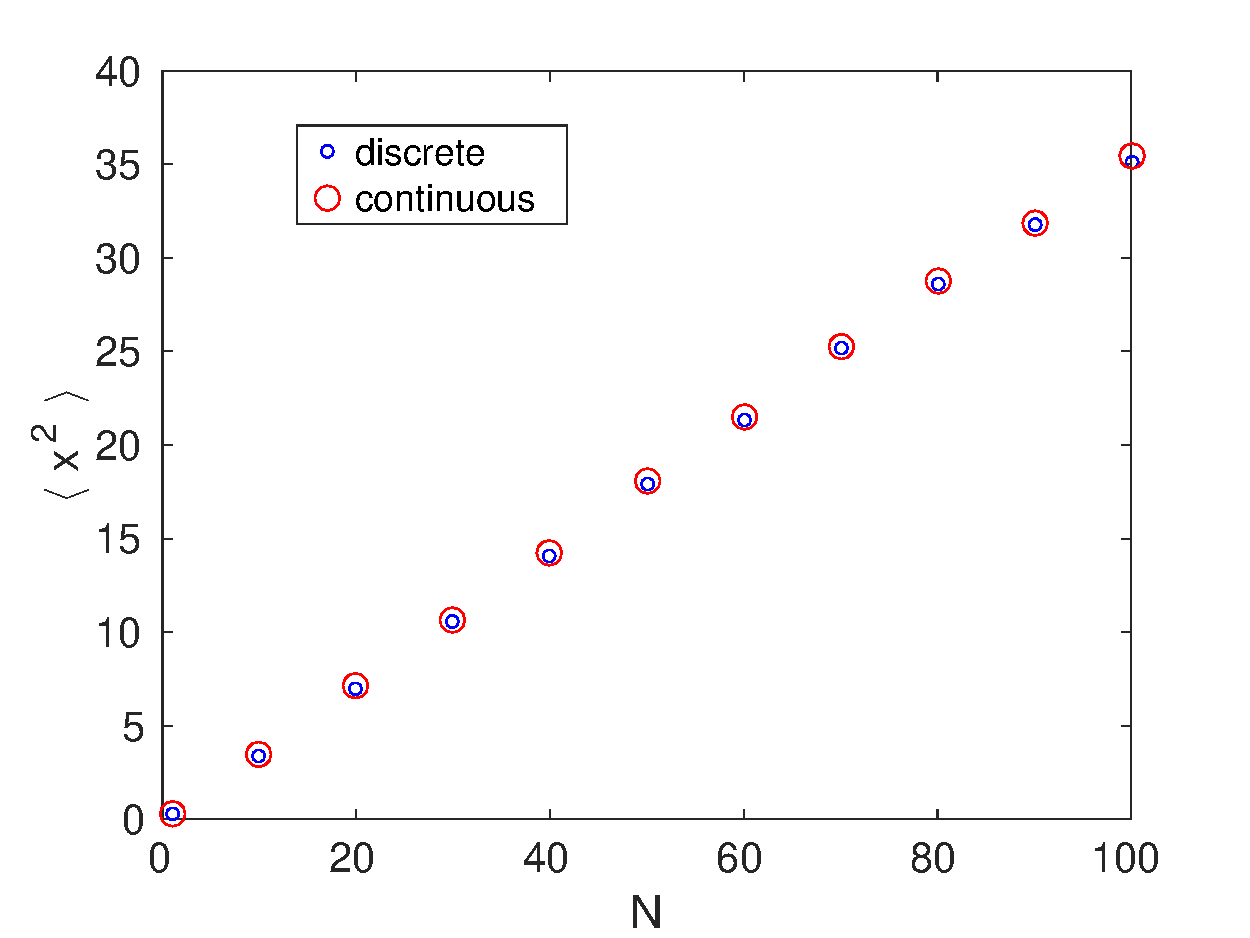
\includegraphics[width=0.5\textwidth]{diffuseDiscreteContinuous}
\caption{Numerical experiment of MSD.  We plot the $\langle x^2\rangle$ as a function of the number of disk collisions. }
\end{figure}